\documentclass[final]{cmpreport}
\RequirePackage{natbib}
\usepackage[utf8]{inputenc}
\usepackage{pgfgantt}
\usepackage{algorithm}   % For math symbols
\usepackage[noend]{algpseudocode}

\title{Progress Report - How can I check?}
\author{James Wright }
\date{October 2021}
\registration{100301701}
\ccode{CMP-6001Y}
\supervisor{Katharina Huber}
\summary{This will be a report detailing on how I designed an application for Students to check their answers to questions based on Linear Algebra and Calculus. It will detail my plans, the features of the application, methodology and then the results of the app. Further analysis will then conclude the success of the planning and methodology.}
\begin{document}
	
	\section{Introduction}
	
	Questions such as "How can I check if my answers are correct?" are on the mind of many students preparing for their assessments. The purpose of this project is to develop a easy-to-use app that will allow students to address this question.\\
	
	In this project, I will initially focus on key concepts arising in linear algebra such as vectors and matrices. Other areas such as calculus and set theory will be included. The target audience are GCSE and A-Level students. My aim is to design a desktop application that has usability and is feature-rich for the target audience. Usability will be judged by syntax recognition and simplicity compared to other sites. \\
	\\This report will detail my planning in the subsection \ref{sec:plan}, then the original design decisions in Section \ref{sec:design1}. I detail any research in my literature review, then my current progress and any issues I have faced, followed by the steps I will be taking next to complete the project. Finally, I will conclude my report with analysis on my progress and planning.
	\subsection{Project Plan}\label{sec:plan}
	In this section, I will be outlining a brief plan as to when to expect certain features within the app to be finished, and any constraints on time that I may need to adjust to. The plan referenced here is shown on a chart in Figure 1.\\
	\\I will start by designing each class as command-line based. I will start with basic classes such as simple algebra. I expect this to be completed by January. Test classes will also be added at the same time. The first class will to implement be the UserInput class detailed in \ref{sec:design} as every other class inherits from it. \\
	\\I will then start doing the GUI, and expect this to be completed by end of February.
	\\Syntax detection and improved user input will follow, expected to be completed by end of March. This will modify the UserInput class detailed in \ref{sec:design}.\\
	\\This leaves 2 months from March for any debugging of errors.\\
	\definecolor{barblue}{RGB}{153,204,254}
	\definecolor{groupblue}{RGB}{51,102,254}
	\definecolor{linkred}{RGB}{165,0,33}
	\renewcommand\sfdefault{phv}
	\renewcommand\mddefault{mc}
	\renewcommand\bfdefault{bc}
	\setganttlinklabel{s-s}{START-TO-START}
	\setganttlinklabel{f-s}{FINISH-TO-START}
	\setganttlinklabel{f-f}{FINISH-TO-FINISH}
	\sffamily
	%
	% A simpler example from the package documentation:
	%
	\begin{figure}[h!]
		
		\begin{ganttchart}{4}{28}
			
			\gantttitle{Weeks}{12} \\
			\gantttitlelist{4,...,28}{1} \\
			\ganttbar{Class Design}{5}{13} \\
			\ganttlinkedbar{GUI Design}{13}{17} \\
			\ganttlinkedbar{Syntax detection}{17}{18} \\
			\ganttlinkedbar{Debugging}{18}{24}\\
			\ganttlink{elem2}{elem3}
			
		\end{ganttchart}
		\label{fig:gantt1}
		\caption{Plan shown by Gantt chart}
	\end{figure}
	\\Since designing this plan a large amount of changes have been made which I have detailed in Section \ref{sec:plan2}. A new Gantt chart was also created in Figure 8.
	\section{Design} \label{sec:design1}
	In this section, we will review design features in Section 2.1, class design in Section 2.2 and a design plan in Section 2.3\\
	\\This will be an application that will be available on all devices that support Python. The GUI will be easy-to-use with multiple categories for different topics. For each topic there will always be an input box to ask for the question (or the question and answer in terms of linear algebra) and then clearly output if the answer was correct or not. If the answer was not correct the app will output the correct answer. The details of some key features are below.\\
	

	
	\subsection{Features}
	The target audience for this application will be aimed at Students, as the majority of users using a site to check answers means they are still learning the topic. Therefore an appropriate set of features for each topic page should make it easy for the user to input a question or answer (depending on the topic) even if they have little prior knowledge of the topic. This application will not only be for elementary students, but also further mathematics students.\\
	\\Features such as linear algebra calculations will involve the manipulation for matrices and vectors while topics related to graphs should have an appropriate graphic to display the graph and any transformations done on it. Graphics showing large images such as a graph, shape or matrix should be scaled appropriately based on it's size. This will allow support for more devices and also make the page a lot easier to read for the user.\\
	\\The most important feature of this application is telling students where they went wrong in their problem solving. A fairly detailed step-by-step solution should be shown for every question. The solutions should be detailed and written in a way that most students can understand. Therefore it is vital that calculations in the solutions use a similar methodology to that used in education systems. This is discussed later in the literature review.\\
	\\The application must show clear syntax formatting as to how the user should input their answer and question. Any minor error by the user should be recognized and corrected by the program.
	
	\subsection{Class Design} \label{sec:design}
	There will be two main stages for the actual design of the application. The first is to produce a set of command-line interface classes that takes an input and can recognize what the question and answer is, and also have a class for syntax formatting. The second stage involves the design of the GUI. I expect Stage 1 to take far longer than Stage 2 due to the vast amount of topics needed to be covered.
	\subsection*{Stage 1}
	Class UserInput: Single class to do basic syntax formatting e.g. $2x+1$ should be the same as $2x + 1$. Classes will be inherited by all other stage 1 classes.\\
	\\All classes below will include use of CLI, each stage of calculation should be printed to console\\
	\\Class NumberFraction: Class to handle user inputting fractions. Should handle fraction to decimal e.g. $4/5 = 0.8$, fraction division: $(4/5)/(2/3) = (3/5)$, simplifying fractions: $(4/10) = (2/5)$, adding of fractions, mixed fractions $(2(4/5))$ etc. Uses of keywords such as ‘simplify’ and ‘multiply’ can be used\\
	\\Class NumberBasic: Deals with prime factor decomposition (‘prime factor 32’), LCM and HCF (‘LCM 2,3,4), surds (simplify root 12), rounding (round 4.374 1dp), converting to standard form(standard form 89000000). Also should deal with any simple adding, subtracting, multiplication and division.\\
	\\Class Algebra: Deals with expanding brackets (expand 4(x+3)), factorisation (factorise $4x+12$), difference of two squares, iteration, solving equations (solve $2x+4=10$), solving simultaneous equations:  \\$(2y + x = 8)$\\$( 1+y=2x)$, solving quadratics, inequalities should be shown on a graph (for now just have a set of points to construct a graph)\\
	\\Class Trigonometry: Recognize the trigonometric functions with sin(x), converts radians to degrees and so forth, for finding edges of a triangle, will have to be given in the form (solve triangle hypotenuse adjacent opposite angle). The side that you want to find can be given as any letter and the side you do not know will be ‘?’ e.g. solve triangle 13 x ? 60. Area of triangle.\\
	\\Class Calculus: Differentiation (should show from first principle aswell), integration
	\\\subsection*{Stage 2 – GUI}
	Class UserInterface: Base screen for original input box and menu selection\\
	\\Class Matrices: Handles a user interface to deal with matrix manipulation. Option to increase size to have variable sized matrices.\\
	\\Class GraphPlotting: This class will be used to construct a graph given a set of points and transform. The syntax for transformations will be the formula you want to do and then the f(x) e.g. transform $(y=x^2+13)$ by $(f(x)+0.5)$.\\
	\\Since making this class design I have created a diagram for it and also changed the class design to add tests in Stage 1 for each class. This can be found in Figure \ref{fig:diag}. An additional stage has also been added but is not detailed in the diagram as the stage is optional.

	\section{Literature Review} \label{sec:lit}
	
	As this is a digital application, I will be reviewing applications with similar goals shown in \ref{sec:intro}, and sites that use syntax formatting to input mathematical questions. The review will be based on it's usability for my target audience and it's features. I will also review sites that were used heavily for research that contributed to the class design.
	
	\subsection{Wolfram Alpha}
	
	Wolfram Alpha \cite{wolfram} is a website that allows you to input an equation and it will display you step-by-step solutions. The solutions is a feature I will be using in a similar manner to Wolfram Alpha. Figure \ref{fig:step} shows an example of quadratic expansion. The important details that makes the solutions easy to read is the simplification of the equation in step 2 to visually show the next step, which then shows each calculation done for the multiplication. Step 4,5 and 6 show each term being added individually and the final answer is clearly displayed in a blue box. \\
	\\My application will improve on that format by including wording to explain the step in a bit more detail. For example step 2 doesn't explain that it is multiplying each term twice in the brackets, meaning that someone who has little knowledge on expanding to polynomials may be confused as to the steps. It is very important that users understand the solutions as the whole point of the application is to educate.
	\begin{figure}[h!]
		\caption{Step-by-step solution for expanding $(x+3)^2$}
		\centering
		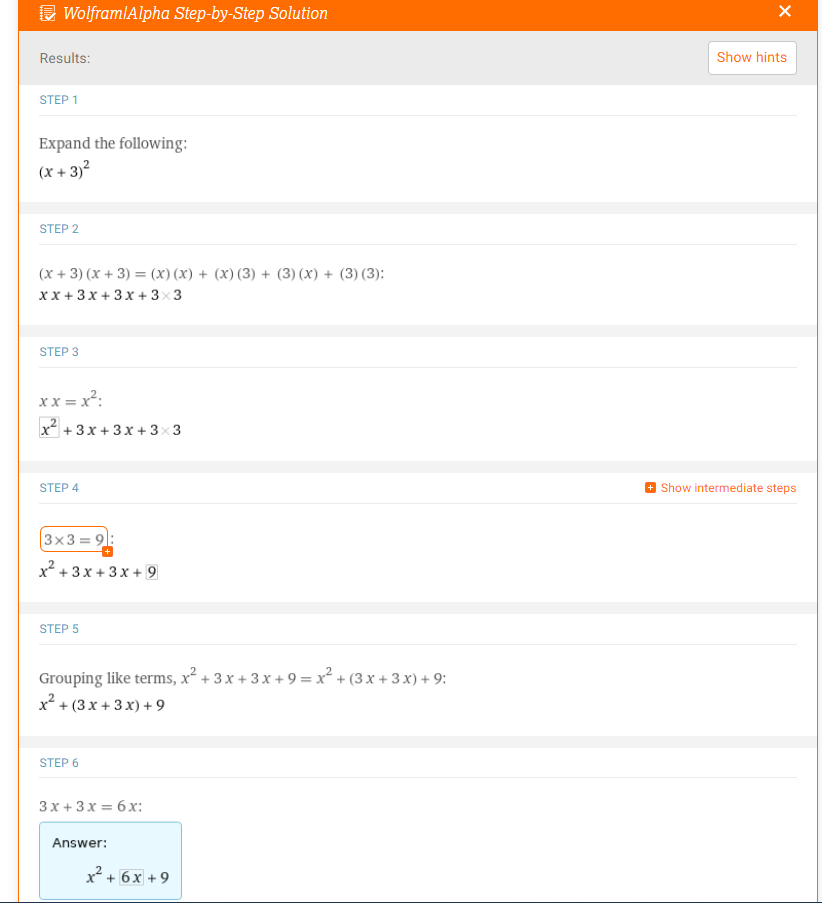
\includegraphics[height=110mm]{step.png}
		\label{fig:step}
	\end{figure}\\
	\begin{figure}[h!]
		\caption{Syntax Formatting. User input box at top of page.}
		\centering
		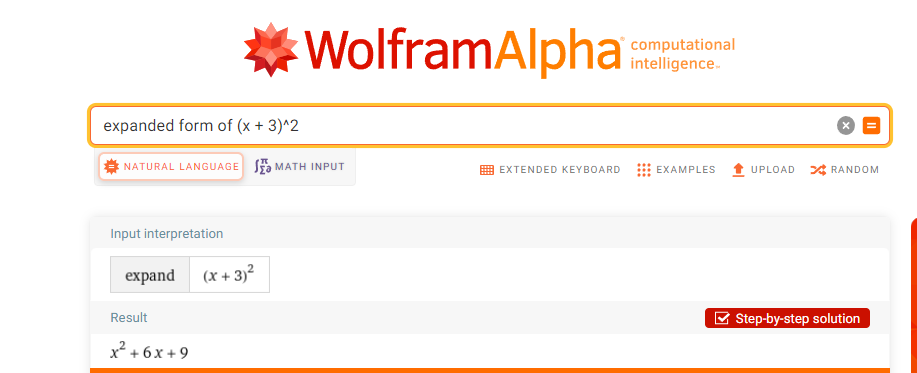
\includegraphics[scale=0.3]{step2.png}
	\end{figure}\\
	The site uses general syntax formatting that is easy-to-use. General syntax formatting means the standard of syntax used for equations worldwide An example of the source's syntax formatting would be using "y''" to show a 2nd order differential for y ($\frac{d^2x}{dy^2} y$). \\
	\\Figure 2 shows the input for figure 1. The wording is used as a command but is very simple for the user and program to recognize. Then $(x+3)^2$ is shown by using a circumflex to display the brackets squared. These are examples of general syntax that I will also be using in my application as well.\\
	\\Visual representations can be given as well. For example simply typing "rotate 30 degrees", will show the rotation matrix and display it visually on a graph.
	Computations of shapes are simply done by specifying parameters and the shape name. For example, "5,12,13 triangle" will display the properties of the triangle with sides of length 5,12 and 13.
	However, the fact I had to go onto help pages and find these examples show more advanced questions are a lot harder. Which is why I will categorize my application to make more specific to what the user is trying to input e.g. for matrices have an input box to visually type the matrix in.\\
	\\In summary, features such as visual representations, syntax formatting and step-by-step solutions will be very similar as to how I plan to design my application. However, it is clear Wolfram Alpha is more aimed at scientific topics that involve heavy mathematics whereas my application is designed more to educate pure mathematics. I will show this by having more detailed step-by-step solutions.\\
	
	\subsection{Microsoft Math Solver}
	
	Microsoft Math Solver \cite{math} is also a website allowing you to input equations and get a detailed output. Figure \ref{fig:output} shows a very basic solution to $ 4 \sin (   \theta     )   \cos (   \theta     )   =  2 \sin (   \theta     )   $. The solution has no wording, no explanation as to how it was calculated and also has variables that are unexplained such as n. The figure also shows a visual representation as a graph which is a feature I plan to include in my application.\\
	\\Figure \ref{fig:topic} shows basic topics on the home page and uses categories of Algebra, Trigonometry and Calculus. The labelling of each topic is easy to understand for a math student. When clicking on a label, there are further options to display what type of equation you want to input. This is better than my original idea of having sub-categories as more pages would be required for something that can fit onto one. I plan on using a similar design in terms of layout for my application.\\
	\\As for the syntax input, the user has a choice to use general syntax or an on-screen keyboard as shown in Figure \ref{fig:calc}. The on-screen keyboard is categorized in order to lower keyboard size but keep as many options to visually input equations. It uses a matrix calculator, algebra calculator, trigonometry calculator and an algebra calculator. Although this will make input easier, it is not something I plan on implementing to my application unless there is spare time. This is because I want the input box to adjust automatically and the calculator's being too difficult for the target audience to use. This would decrease the software's usability.\\
	\begin{figure}[h!]
		\caption{Answer output. Input box at top of page, with $\theta$ being equal to the input solution. Also a graph below of the function. }
		\centering
		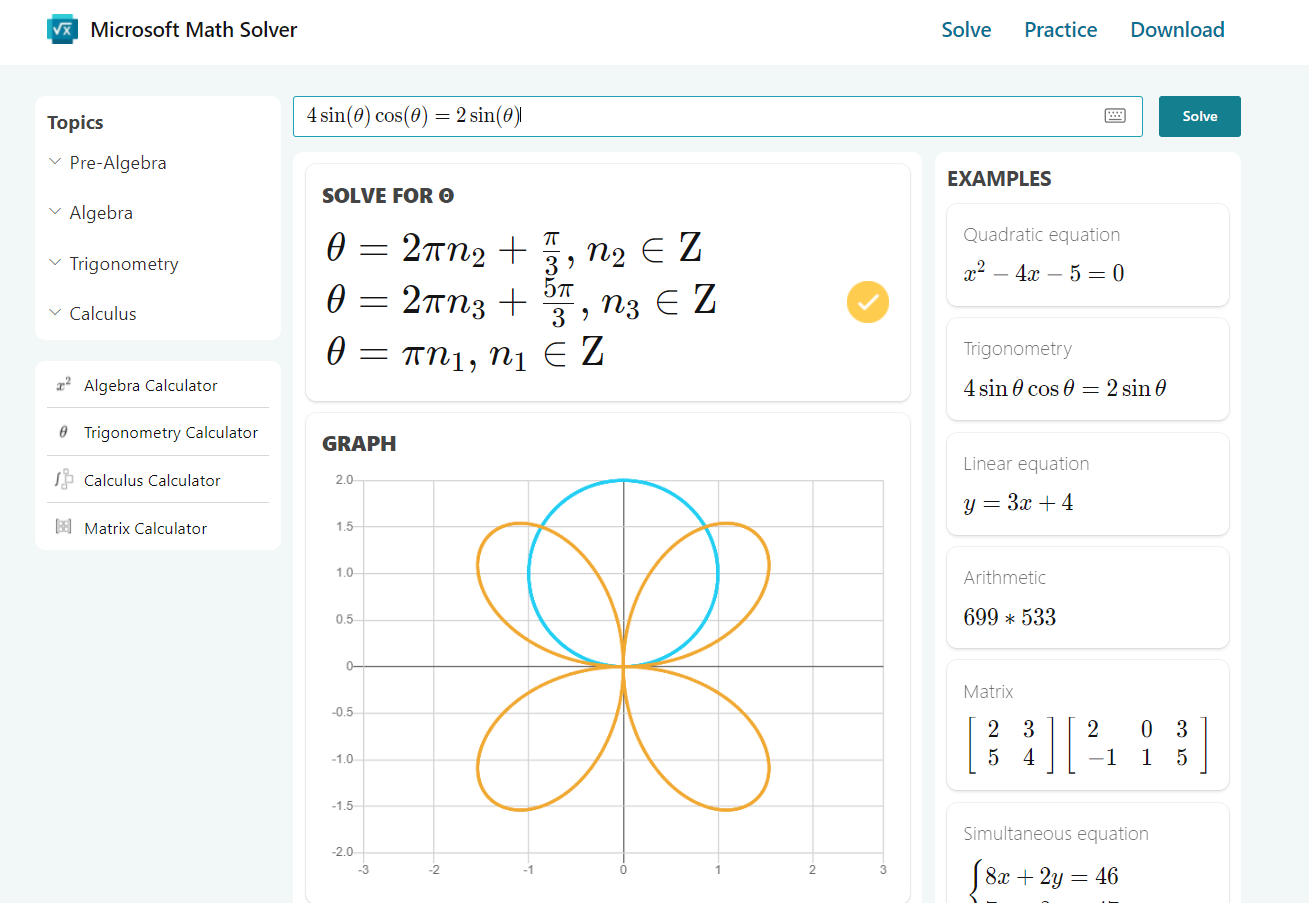
\includegraphics[scale=0.4]{mathsolver3.png}
		\label{fig:output}
	\end{figure}
	\begin{figure}[h!]
		\caption{Topics split into sections found in the A-Level Curriculum}
		\centering
		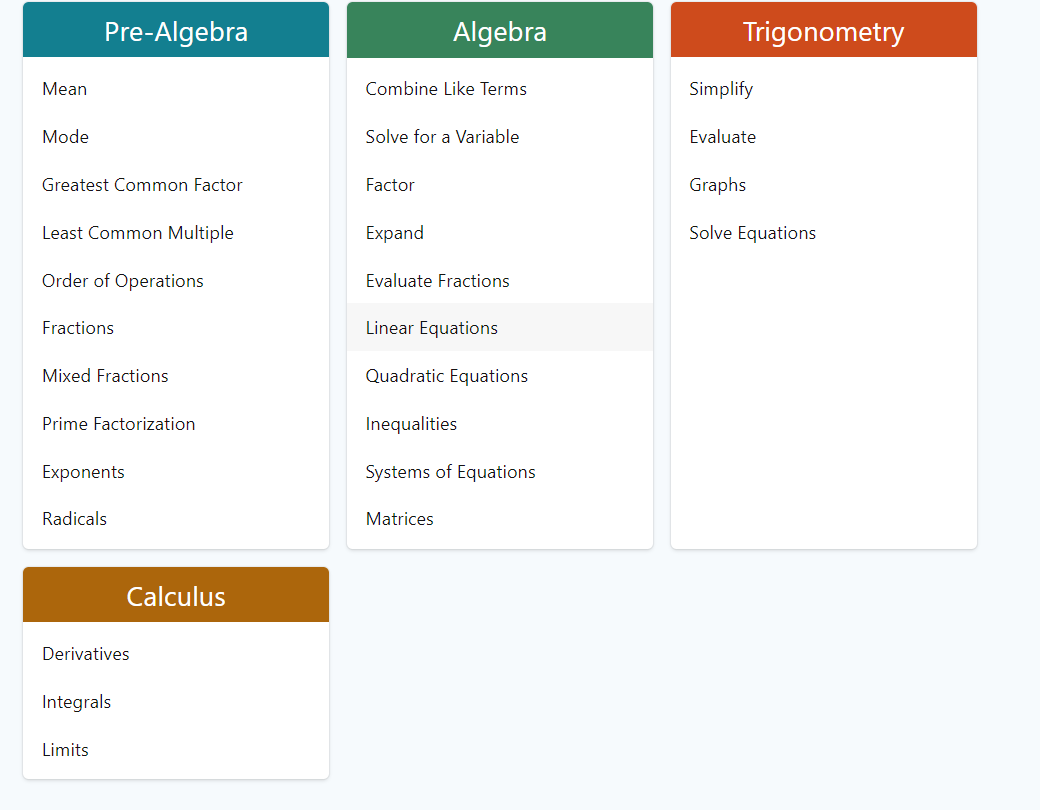
\includegraphics[scale=0.3]{mathsolver2.png}
		\label{fig:topic}
		\end{figure}
	\begin{figure}[h!]
		\caption{Calculator Input}
		\centering
		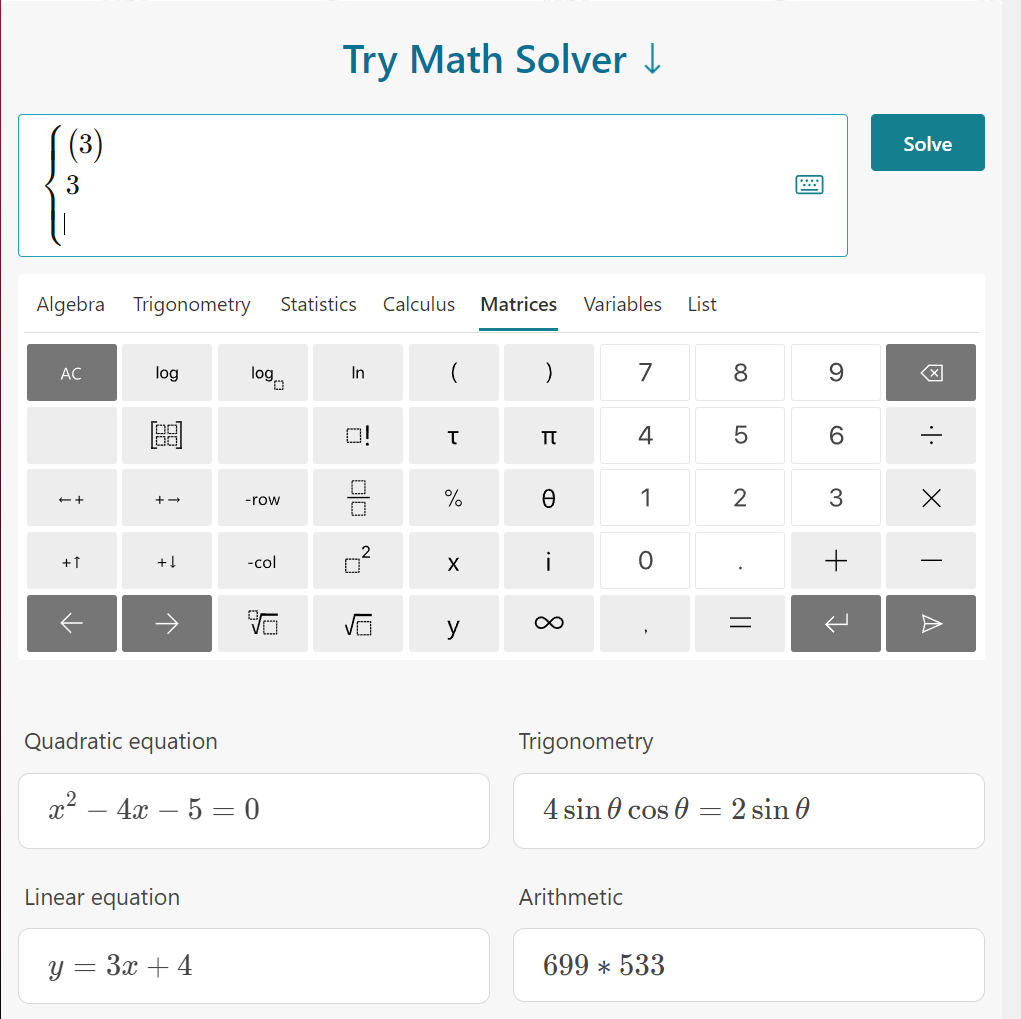
\includegraphics[scale=0.3]{mathsolver.png}
		\label{fig:calc}
	\end{figure}
	
	
	
	\subsection{Revision Maths}
	
	Revision Maths provides GCSE and A-Level revision materials for mathematics. \cite{revision}.This source will be used to decide which topics of mathematics I need to include. I have picked ones I believe are of key importance and tried to include most topics from the GCSE and A-Level curriculum to make it realistic for a student to be checking their answer.\\
	\\This site was mainly used for the class design in Stage 1. I also plan to use this source later on when implementing the classes to better understand the mathematics before programming. For example, matrix manipulation is something I plan to educate myself on before even starting to write the code. In fact, I designed a few algorithms after educating myself on matrices shown in Section \ref{sec:prog}. This website will be my main source for learning the mathematical methods in order to design more pseudocode. \\
	
	\section{Current Progress}\label{sec:prog}
	This section will detail the completion of my planning, literature review and class design. It will also detail extra research done on programming and any other work that has contributed to the project. To note why some research wasn't in the literature review is because this was done after I completed \ref{sec:lit} or the research wasn't substantial enough.
	\\I completed the planning stage for my project on December 10th. This was later than expected and as a result have had to change my plan (which is discussed later in the report). Research into IDE's and programming languages has allowed me to position myself well to start the programming after December 15th. The language I settled on was Python and the IDE is PyCharm. I will use Python version 3.9 due to being already up to date on the API documentation.\\
	\\Choosing a Python library for the GUI proved to be trickier than I had thought. Originally I planned to use a GUI library called Tkinter, but after further research, it would be a lot easier to implement a smoother design with a library called PyQt6. I read up on the documentation and chose this library due to it's ease of use. \cite{pyqt}\\
	\\A lot of class design and the literature review was already done on my project proposal. Since then, I have done further research on topics and edited my class design. \\
	\\As a result of the mathematical study, I constructed a few algorithms for matrix manipulation and linear algebra. Algorithm 1 shows the pseudocode I created for multiplying two matrices while algorithm 2 shows the pseudocode for adding two matrices. Further algorithms will be found in the notebook. Writing pseudocode should make the mathematical side of the programming a lot easier and less time-consuming.
	\begin{algorithm}
		\caption{Round Matrix}
		\begin{algorithmic}[3]
			\Procedure{RoundArr}{$arr,d$}
			\State $multiplier \Leftarrow 10^d$
			\State $arr \Leftarrow matrix[n>=1][n>=1]$
			\For {i in $arr[0]$}
			\For {j in $arr[1]$}
			\State $arr[i][j] \Leftarrow (arr[i][j]*multiplier)/multiplier$
			\EndFor
			\EndFor
			\Return $arr$
			\EndProcedure			
		\end{algorithmic}
	\end{algorithm}
	\begin{algorithm}
		\caption{Matrix multiplication}
		\begin{algorithmic}[1]
			
			\Procedure{multiplyMatrix}{$a,b$}  
			\State $result \Leftarrow matrix[$length $a, $length $a +1] $
			\For {i in length $a}$
			\For{j in length $b[0]}$
			\For{k in length $b}$
			\State $result[i][j] \Leftarrow result[i][j] + a[i][k]*b[k][j]$
			\EndFor
			\EndFor
			\EndFor
			\Return $result$
			\EndProcedure
		\end{algorithmic}
	\end{algorithm}
\begin{algorithm}
	\caption{Matrix Addition}
	\begin{algorithmic}[2]
		
		\Procedure{addMatrix}{$a,b$}  
		\State $result \Leftarrow matrix[$length $a, $length $a] $
		\If{length $a == $length $b}$
		\For {i in range length $a}$
		\For{j in range length $b}$
		\State $result[i][j] \Leftarrow a[i][j]+b[i][j]$
		\EndFor
		\EndFor
		\EndIf
		\Return $result$
		\EndProcedure
	\end{algorithmic}
\end{algorithm}
	\section{Issues encountered and mitigation}
	In this section, I will discuss the several issues I faced with achieving my plan and class design. Mainly, considerations of usability and time constraints is what lead to the discovery of the issues. I will then address the changes I made in order to achieve my objectives stated in the Introduction and project outline.
	\subsection{Class Design Issues}
	I had planned to begin programming in Week 12 as shown in the planning Section \ref{sec:plan}. The class design was a textual concept of the classes giving a brief description of it's features. Defining variable names or inheritance was not done in the design phase as idea was to add more to the class design as I programmed more. However, this was quickly proven to be a bad idea as class design was needed to layout the topics and what the classes should have. Furthermore, I wanted to design a few algorithms before coding.\\
	\\The original class design may be too big in Stage 1 to be completed in time. Therefore I removed a few classes that are not as important to my objective. For example, graphing and trigonometry are not as vital as basic linear algebra and matrix manipulation. Hence, I added a Stage 3 which contains classes that are not needed, but if some stages took less time than expected, Stage 3 will be the final stage in my plan. The classes Trigonometry and Calculus were moved from Stage 1 to Stage 3, and GraphPlotting from Stage 2 to Stage 3.\\
	\\I also noticed that my class design was inconsistent across stages. For example the class Matrices, should also be in Stage 1, where the functions for matrix manipulations should already be created. Then in stage 2, I will create the user interface features for it.\\
	\\My design had not accounted for testing my software. For each class, there should be a test class and I decided I should make these test classes after finishing each class. Therefore, I can structure my code around sufficient testing to make for easier debugging.\\
	\\Due to the amount of changes I made to my class design I constructed a very simple class diagram. This is shown in Figure \ref{fig:diag}. I chose not to add the classes in Stage 3 as the default is not to add them.
	\begin{figure}[h!]

		\caption{Class Design}
		\hspace*{-2cm}
		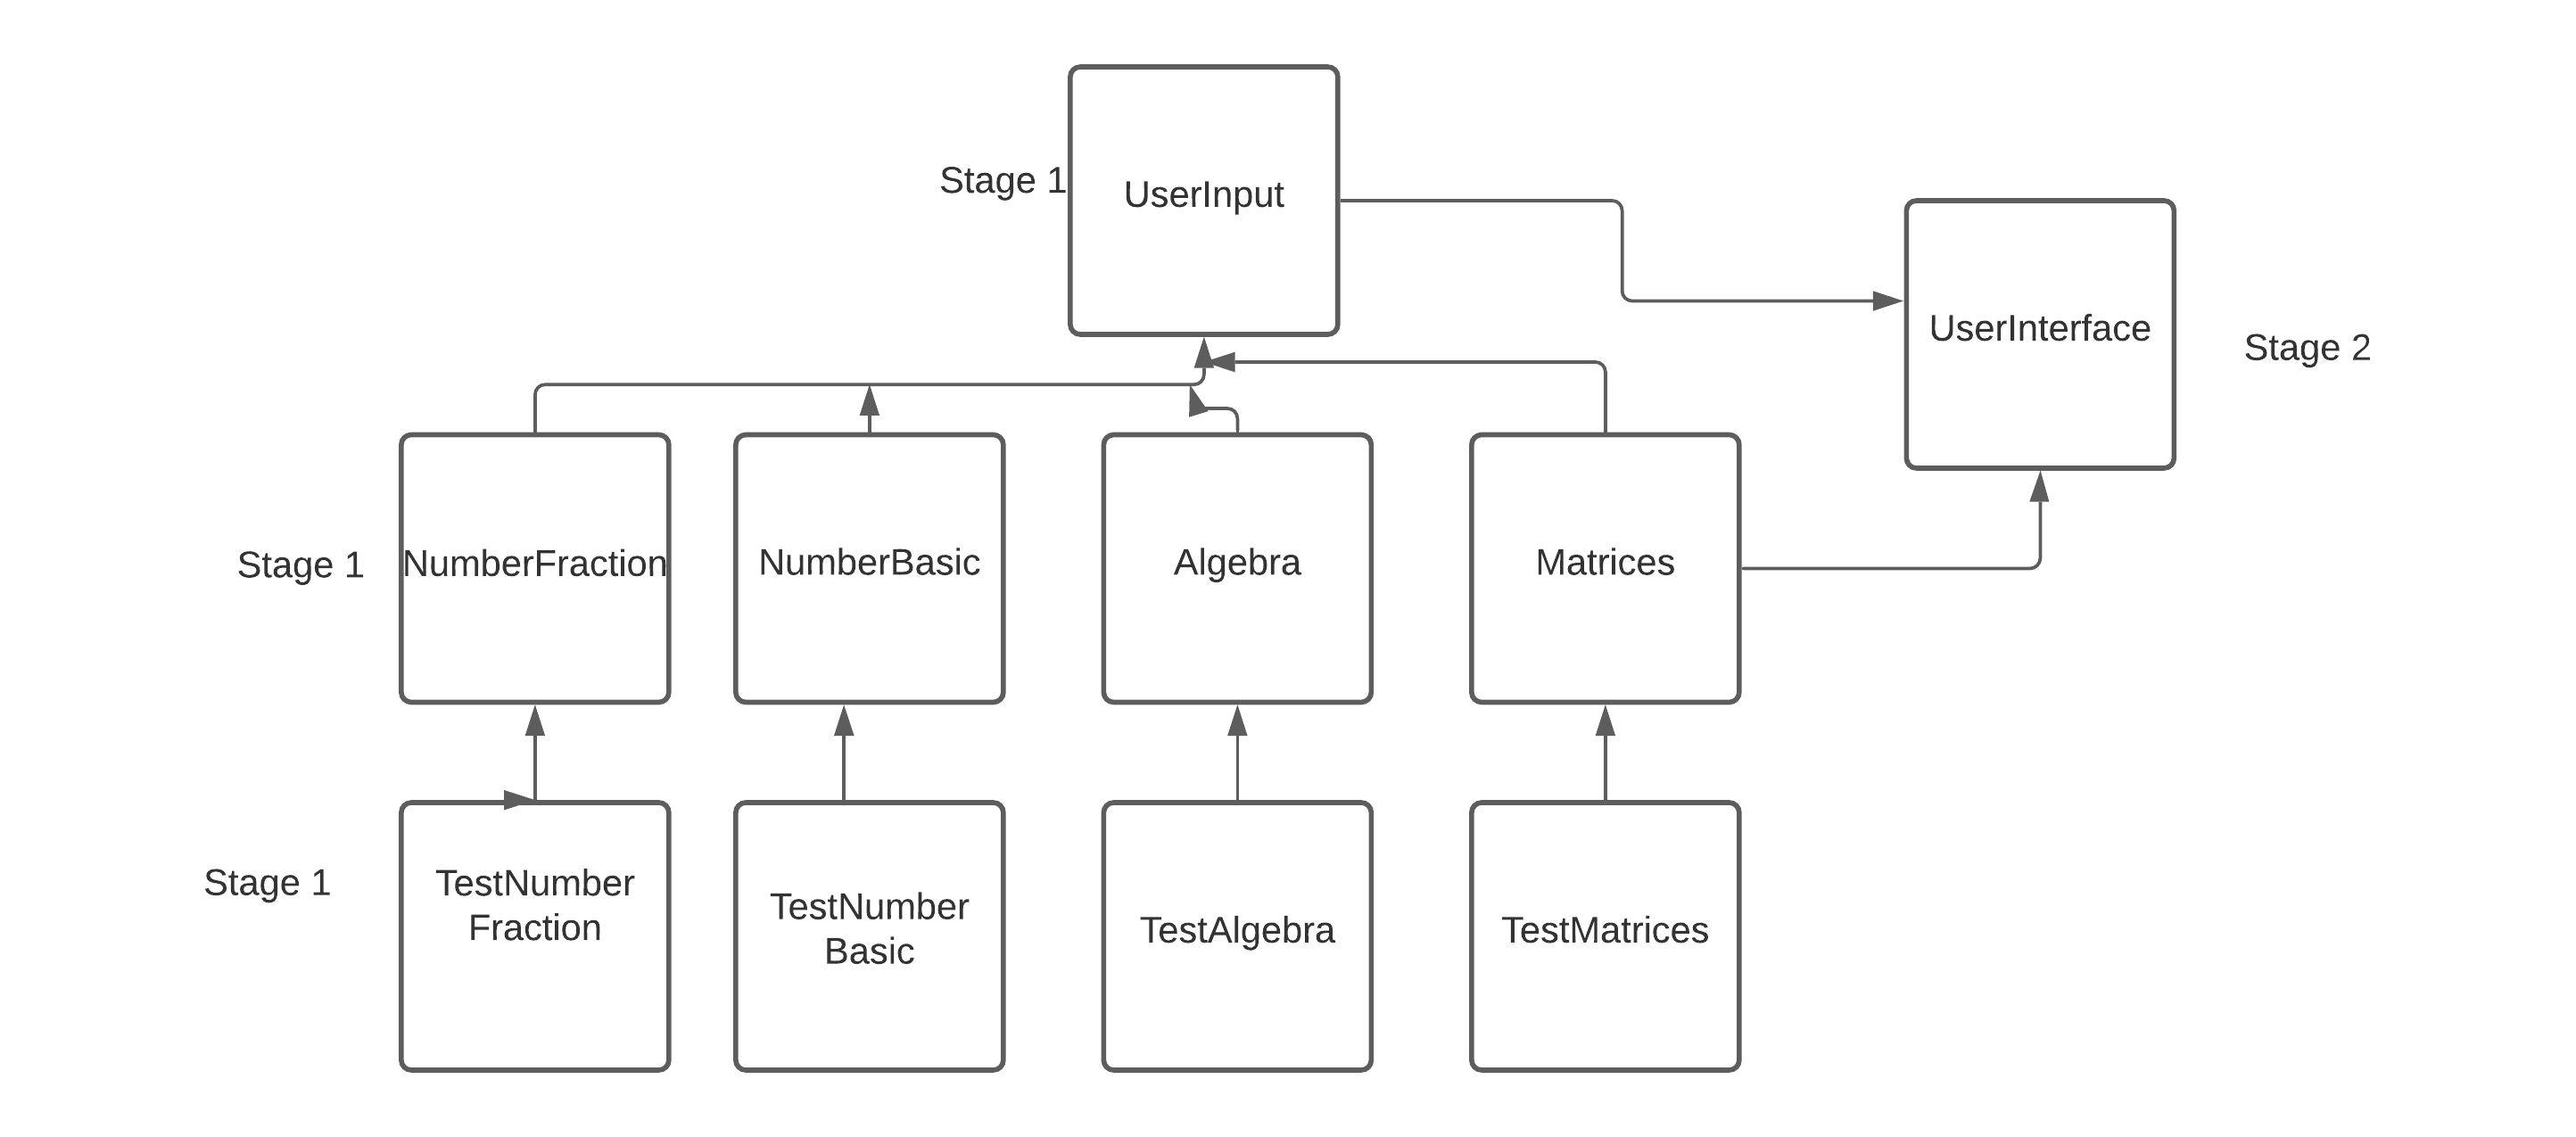
\includegraphics[scale=0.8]{diag.png}
		\label{fig:diag}
	\end{figure}
	\subsection{Planning Issues}\label{sec:plan2}
	
	I constructed my plan based on the number of weeks since the start of the project to the due date. This was because having set dates was unrealistic as I am unable to know exactly how long each class will take. Figure 1 shows that class design should be completed by now. However, I misunderstood class design as being the design and implementation. Therefore, my plan failed to separate the implementation stages in my class design.\\
	\\Due to the original plan already not being met and failing to account for many stages of development, I created a new plan as shown in Figure 8. This plan accounts for the literature review and class design already done (with changes made). It then states that the implementation should be started by Week 12, which is the time I currently plan to begin.\\
	\definecolor{barblue}{RGB}{153,204,254}
	\definecolor{groupblue}{RGB}{51,102,254}
	\definecolor{linkred}{RGB}{165,0,33}
	\renewcommand\sfdefault{phv}
	\renewcommand\mddefault{mc}
	\renewcommand\bfdefault{bc}
	\setganttlinklabel{s-s}{START-TO-START}
	\setganttlinklabel{f-s}{FINISH-TO-START}
	\setganttlinklabel{f-f}{FINISH-TO-FINISH}
	\sffamily
	%
	% A simpler example from the package documentation:
	%
	\begin{figure}[h!]\label{fig:Gantt Chart 2}
	
	\hspace*{-3cm}
	\caption{New plan in form of Gantt Chart}

	\begin{ganttchart}{4}{28}
		
		\gantttitle{Weeks}{12} \\
		\gantttitlelist{4,...,28}{1} \\
		\ganttbar{Literature Review}{4}{8}\\
		\ganttlinkedbar{Class Design}{6}{12} \\
		\ganttlinkedbar{Stage 1 implementation}{12}{20}\\
		\ganttlinkedbar{Stage 2 implementation}{20}{25} \\
		\ganttlinkedbar{Syntax detection}{25}{26} \\
		\ganttlinkedbar{Debugging/stage 3 classes}{26}{28}\\
		\ganttlink{elem2}{elem3}
		\ganttlink{elem3}{elem4}
		
	\end{ganttchart}
	\end{figure}
	\\The new plan splits up the stages of implementation as some will take longer than others. Therefore setting a goal for Stage 1(which I expect to take the longest) and stage 2 allows me to analyse how much time I have left. The fact I already have a lot of pseudocode to use, stage 1 may take a lot less time than expected, which is why I added an optional Stage 3. \\
	\\I expect stage 2 to be completed in 13 weeks. By then the program should be usable, and the extra time I have is for debugging and adding in the classes of Stage 3. Syntax detection is optional like Stage 3, but I would work on this feature before then as the usability of the program is more important than extra features. The time taken for debugging is expected to be lower due to test cases now being included in the stage implementation.
	
	\section{Results} \label{sec:results}
	
	In this section I will be detailing the results obtained through the methodology. The main result in the final program will be the GUI (Graphical User Interface) in which the client will be using. Upon using this GUI, users can carry out mathematical operations and receive a result verifying if their answer is correct. This achieves the goal of my project in the question of a student - "How can I check?"
	
	The starting screen of the program can be seen in Figure **. The options are simple and categorised for maths students. The choice of a vectors and matrix section can be seen in a frame, and a simultaneous equations button with a list box option to choose the number of unknowns. A further feature is added for selecting the program's theme. This window is clear and concise for any student to use which is why I chose this layout.
	
	\subsection{Matrices} \label{sec:matrices}
	
	Upon the user pressing on the matrices button, they will see a variety of matrix operations to carry out. This is shown in Figure **. There are 2 frames, one for single matrix operations and the other for double matrix operations. For each operation, the dimensions can be selected next to the button, aside from matrix multiplication which has a separate page for selecting the dimensions. 
	
	The reason for this is to make it less complicated for the student, as this is the only operation that requires two matrices of two different dimensions. The selection screen can be seen in Figure **. For Matrix Multiplication, the dimensions have to be specific for the operation to work. If both matrices are of dimension $m * n$, the $m$ of the first matrix must equal the $n$ of the second matrix. If this condition is not met, a pop-up window is created warning the user.
	
	\subsection{Matrix Inverse} \label{sec:inv}
	
	An example of a matrix operation that has a feature other programs do not have is finding the inverse of a matrix. This will tell the user each step carried out in the operation, which is especially helpful for inverting a matrix as there are several steps that involve other operations on the matrix screen.
	
	As can be seen in Figure *, to input the matrix a set of boxes are laid out and the user is free to input decimals or a whole number. The help bar will also notify the user they can press the TAB button in order to quickly input data without the need for mouse movement. Upon pressing the "Solve" button the user is then told the steps in the output box below. The first step is to find the determinant and inform the user of it. Then the matrix of minors is calculated, followed by applying the matrix of cofactors to it. Then it is transposed, and the result is displayed clearly to the user.
	
	This is a very useful feature as all of these operations are in the matrix section of the program, allowing the user to see where they went wrong. However, as not all matrices cannot be inverted, the user will be told why the matrix cannot be inverted and what the determinant is as can be seen in Figure **.
	
	
	
	

	\section{Conclusion}
	To summarise this report, I had an original plan that didn't take into account of quite a few aspects of the software, which also wouldn't fulfil my class design. Due to a lack of testing, test classes had to be added to Stage 1 of the class design, then some classes were removed due to time constraints caused by the planning issues. I adjusted the plan to make sure that usability is a priority over extra features by allocating more time to the Stage 1 phase and adding an optional phase for implementation.\\
	\\My literature review has been very helpful to get a good idea of the features of my software and aided in writing a few algorithms. I also have decided my programming environment. With class design, algorithms for these classes and a proper plan in place, it puts me in a very good place to start development of the software and complete the next steps. \ref{sec:step}\\

	\newpage
	\section*{Appendix..Notebook}\label{app:a}
	\begin{enumerate}
		\item[$\bullet$] Week 4: Set up meetings every 2 weeks with supervisor.
		Project proposal started. Considered target audience as students. Focus is on usability as talked about in the introduction.
		\item[$\bullet$] Week 5-6: Topics decided after research from \cite{math}
		Features written in proposal. Step-by-step solutions emphasised. Used sources wolfram alpha and Microsoft math solver.
		Simple class layout created in a textual layout. Specific features added. No need to define variables or methods as some methods may have a module.
		Created two stages to the class design.
		Created gantt chart over 28 weeks as plan.
		Feature of graphing added to proposal and class design.
		\item[$\bullet$] Week 6-8: Literature review completed
		Research into Java GUI. Features considered from 
		Decided to use Python 3.9 and PyQt6 due to the complexity of Java GUI in relation to python gui libraries. 
		Brief research into ease of use for PyQt6.\cite{pyqt}
		Started project progress report	
		Considering graphical features such as input box and calculator layouts. Decided not to use calculator layouts due to complexity. Should input box automatically adjust size or have different pages with different input boxes? 
		\item[$\bullet$] Week 8-10: Started writing pseudocode for functions that didn’t already have a module in python. See Figure \ref{fig:psudo}. Meeting setup with supervisor day before due date
		\begin{figure}[h!]
			
			\caption{Algorithms containing methods for finding the lowest common multiple and prime factor}
			\centering
			\hspace*{-2cm}
			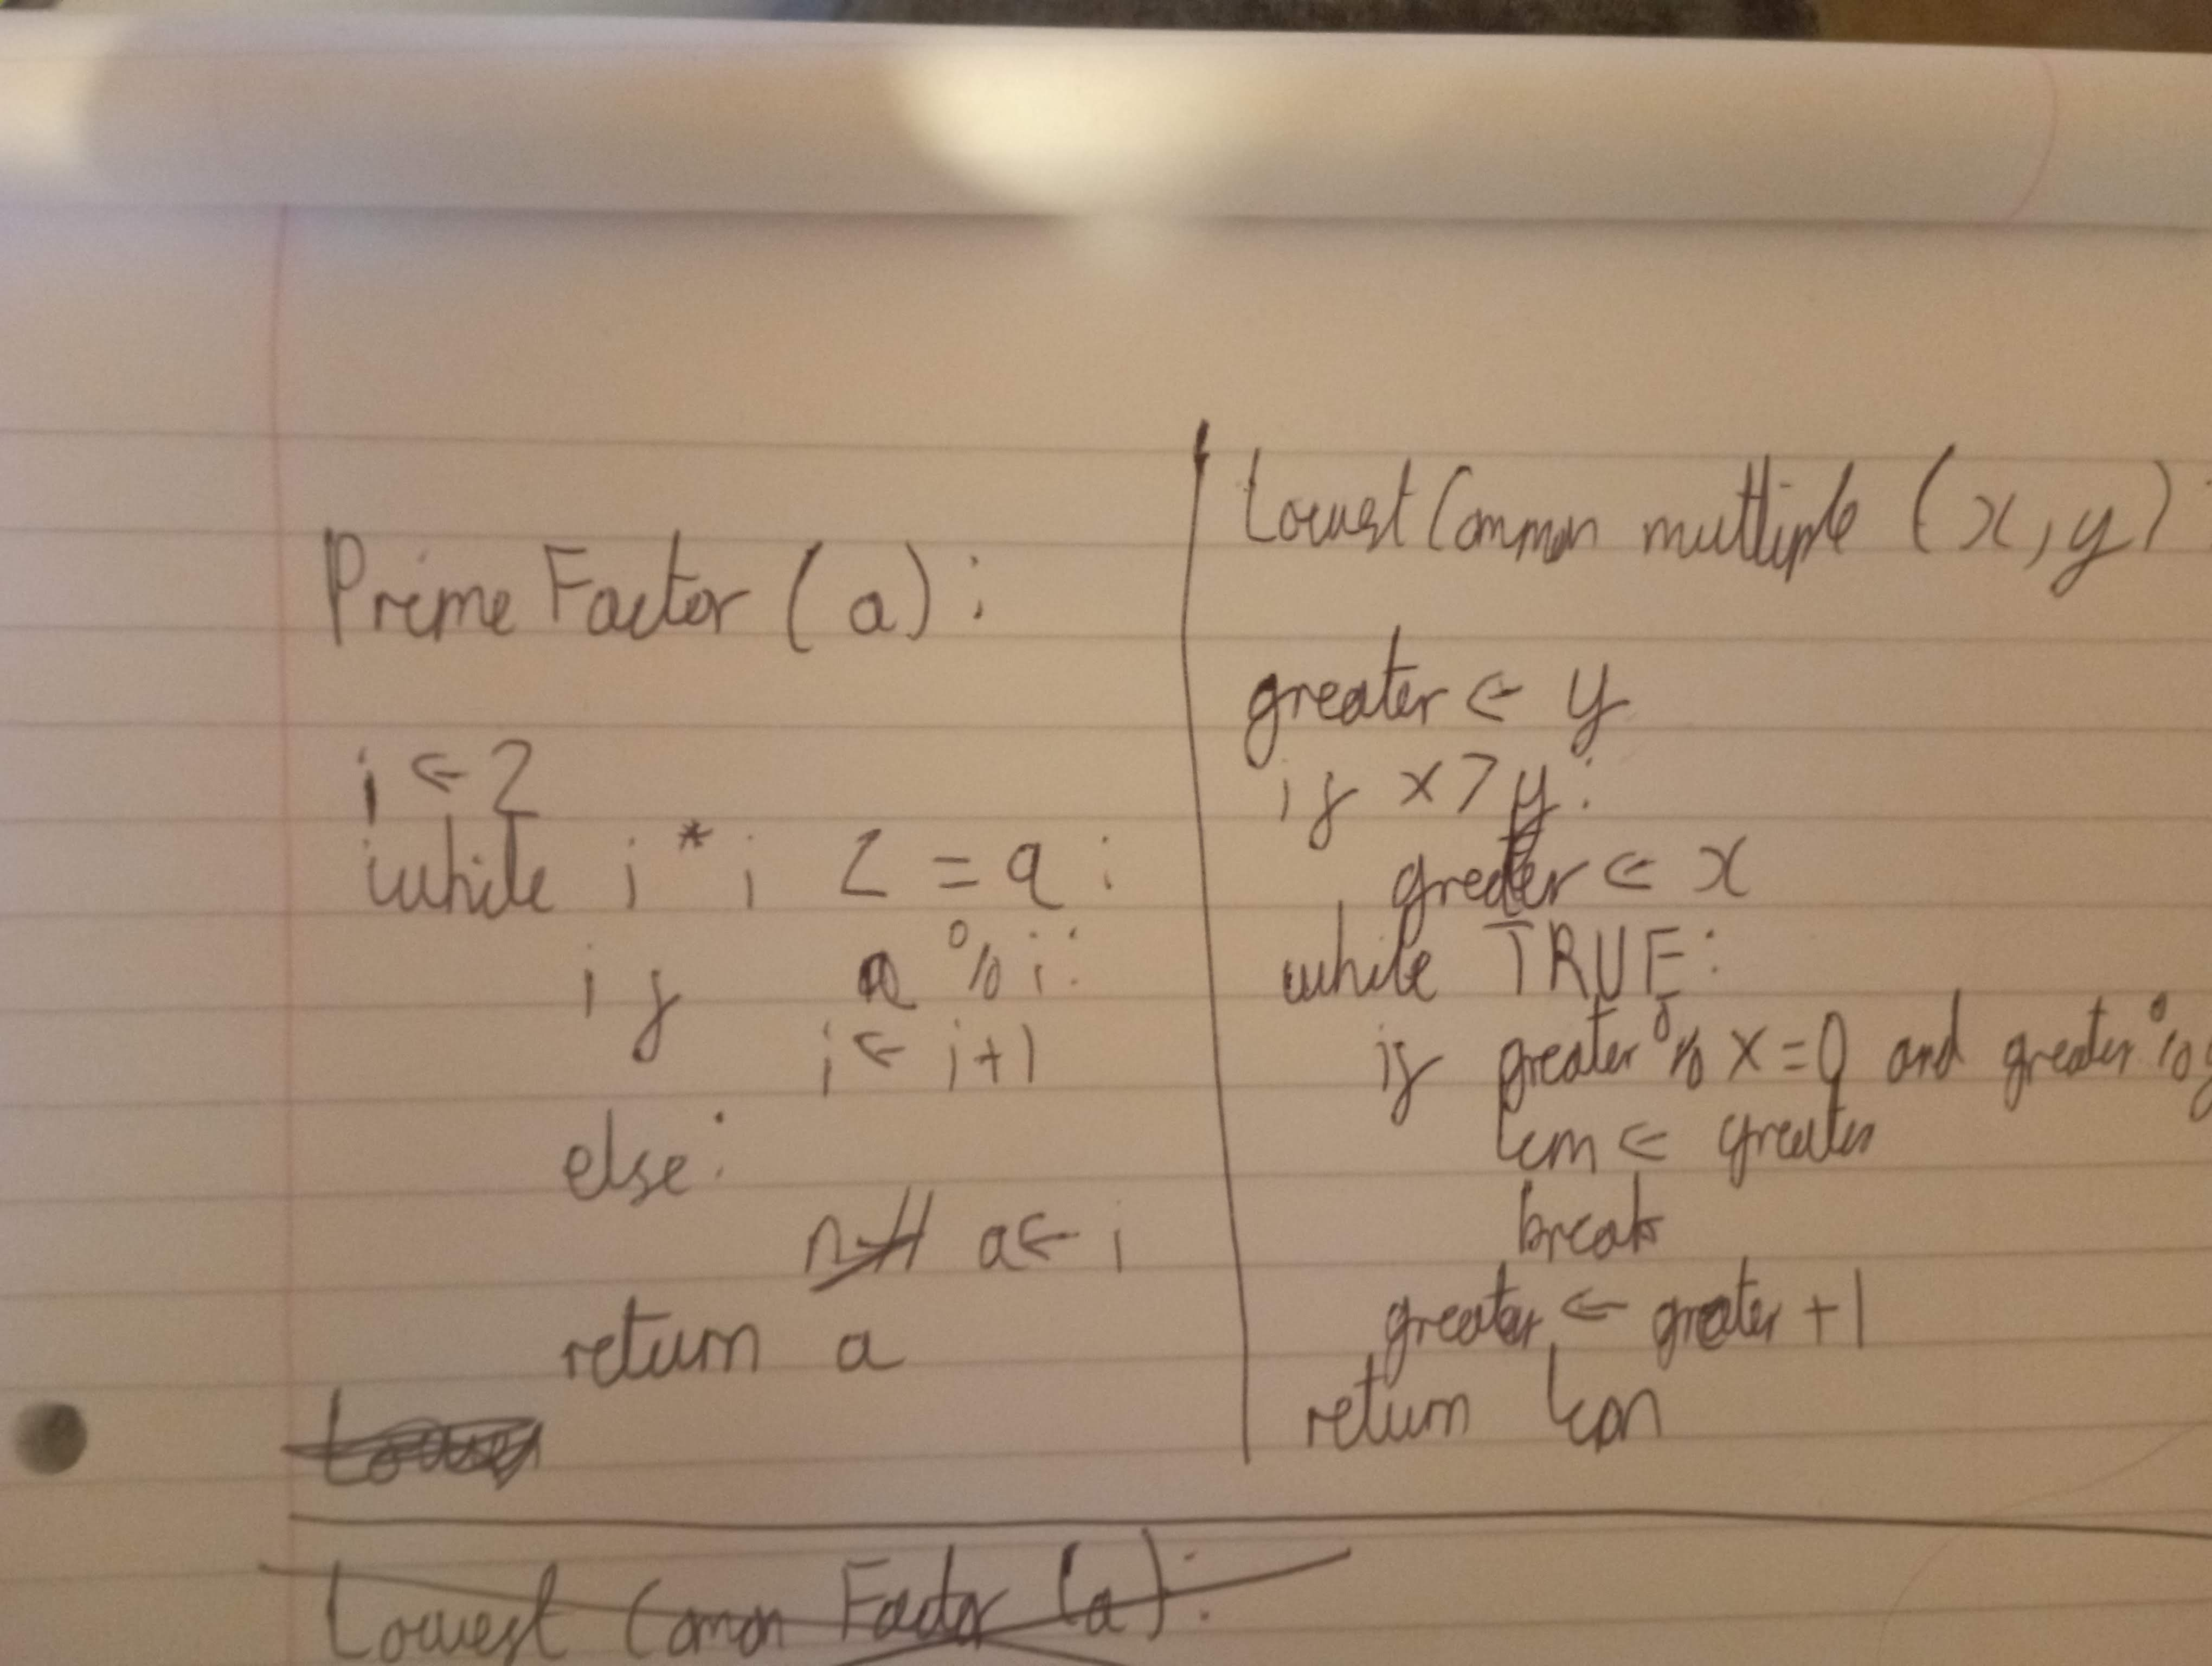
\includegraphics[scale=0.1]{psudocode.jpg}
			\label{fig:psudo}
		\end{figure}
		\item[$\bullet$] Week 10-12: Stage 1 is far too big. Removed class calculus, graphing, trigonometry and moved them to stage 3
		Stage 3 is going to be optional if I have enough time at the end.
		Testing has not been considered. Add in test classes to the class design.
		Construct class diagram. Will all classes inherit UserInput?
		New plan constructed to adjust to class diagram. Plan needs extra sections for stage 1 and 2 as misunderstood what class design meant.
		Completed project report. 
		
		
		
		
		
	\end{enumerate}
\newpage
	\bibliographystyle{apalike}
	\bibliography{myBib.bib}
\end{document}
